\documentclass[draft]{article}
\usepackage[utf8]{inputenc}
\usepackage{listings}
\usepackage{color}
\usepackage{graphicx}
\usepackage{supertabular}
\usepackage{booktabs}
\usepackage{caption}
\usepackage[table,xcdraw]{xcolor}
\usepackage{color}
\usepackage{courier}
 
\definecolor{codegreen}{rgb}{0,0.6,0}
\definecolor{codegray}{rgb}{0.5,0.5,0.5}
\definecolor{codepurple}{rgb}{0.58,0,0.82}
\definecolor{backcolour}{rgb}{0.95,0.95,0.92}
 
\lstdefinestyle{mystyle}{
    backgroundcolor=\color{backcolour},   
    commentstyle=\color{codegreen},
    keywordstyle=\color{magenta},
    numberstyle=\tiny\color{codegray},
    stringstyle=\color{codepurple},
    basicstyle=\footnotesize,
    breakatwhitespace=false,         
    breaklines=true,                 
    captionpos=b,                    
    keepspaces=true,        
    language=Python,
    numbers=left,                    
    numbersep=5pt,                  
    showspaces=false,                
    showstringspaces=false,
    showtabs=false,                  
    tabsize=4
}
 
\lstset{style=mystyle}

\title{Chapter 5 - Experimentation (Draft)}
\author{Michael Neary}
\date{November 2018}

\begin{document}
\maketitle
This chapter discusses the methods of experimentation that are used to analyze student solutions to programming problems, including the human labelers, their qualifications, and their overall agreement on the data sets.

\section{Data}
The data that I use to test my method of extraneous code detection originates from the Computer Science I for Majors (CMSC 201) course at the University of Maryland, Baltimore County (UMBC). This is the first course in programming, required for Computer Science majors at the university. The course is taught in Python, a suitable beginner's programming language. It is assumed that the students in this course do not have prior programming experience. Homework assignments during this semester were given weekly, with four to seven individual problems. I have collected several hundred code samples for two different problems that were given as homework assignments during the Fall semester of 2016. Each of these problems have been selected for their simplicity; they can be solved by applying a few fundamental programming structures. The following paragraphs are short descriptions of each of the problems used in this work.

\begin{figure}[ht]
\begin{lstlisting}[numbers=none]
def main():
    temp = float(input("Please enter the temperature: "))
    unit = input("Enter 'C' for Celsius, or 'K' for Kelvin: ")
    if unit == "K":
        temp -= 273.15
    
    if temp >= 100:
        print("At this temperature, water is a gas.")
    elif temp <= 0:
        print("At this temperature, water is a solid.")
    else:
        print("At this temperature, water is a liquid.")

main()
\end{lstlisting}
\caption{A correct solution for Problem 1.}
\label{fig:correctp1}
\end{figure}

\subsection{Problem 1: State of Matter}\label{p1desc}
The goal of this problem is to output the state of matter that water would be in at a certain temperature. This problem asks the student to accept two inputs from the user: a floating point number that represents a temperature, and a character to determine what unit that temperature is in (`C' for Celsius or `K' for Kelvin). Their program must output the state of matter that water would be in at the given temperature. Acceptable output should contain one of the following strings: `liquid', `solid', or `gas.' The output format was not strictly enforced, as long as it produced the correct string for the given input. An appropriate solution uses two input statements, followed by a sequence of condition statements, to produce correct output. Refer to Figure \ref{fig:correctp1} for a correct solution, bearing in mind that this problem's complexity gives rise to many different methods of solving this problem.

\begin{figure}[ht]
\begin{lstlisting}[numbers=none]
def main():
    width = int(input("Enter the width of the box: "))
    height = int(input("Enter the height of the box: "))
    outline = input("Enter a symbol for the box outline:")
    fill = input("Enter a symbol for the box fill:")

    for i in range(width):
        print(outline, end = "")
    print()
    
    if height > 1:
        for i in range(height - 2):
            print(outline, end = "")
            
            if width > 1:
                for j in range(width - 2):
                    print(fill, end = "")
                    
                print(outline, end = "")
            
            print()

    for i in range(width):
        print(outline, end = "")
    
    print()

main()
  \end{lstlisting}
  \caption{A correct solution for Problem 2.}
  \label{fig:correctp2}
\end{figure}

\subsection{Problem 2: Box Display}\label{p2desc}
The goal of this problem is to display a rectangular box on the screen constructed with any character on the keyboard. The problem asks the student to accept two integer inputs that represent the height and width of the box, one character input that fills the inside of the box, and one character input that makes up the border of the box. Their program must output a box with the given dimensions, constructed with the given characters in the correct places. A student must combine multiple programming structures to give a correct output as they must consider a few edge cases in order to produce a correct solution. Refer to Figure \ref{fig:correctp2} for a correct solution.

\subsection{Data Preprocessing}
Each of the data sets must be standardized before my extraneous line detection method is evaluated. Standardization of each file helps streamline the process of labeling the extraneous lines, both manually and automatically. The contents of each file in the same assignment group are different for each student, but the name of each submitted file is the same within each data set (i.e., hw3.txt). To distinguish between unique solutions within each data set, every file name is appended with a different number (hw3\_123.txt). Every file is stripped of the file header and comments to protect the identity of the student who submitted that file. Identity was not preserved between the datasets, meaning that hw3\_123.txt and hw5\_123.txt may not be the same student's code. All blank lines are removed from the file to remove the possibility of reporting such lines as extraneous. All empty files are removed from the dataset.

\section{Data Labeling}

Each individual assignment must be manually checked for extraneous lines of code in order to properly evaluate my detection method. In other words, a baseline of ``true labels'' that describe whether or not a line of code is extraneous needs to be created in order to understand if this detection method is valid. This process involves reading through each program line by line, scanning for lines of code that do not make sense or do not help the student solve the problem. This is a simple task that I could perform on my own, so I independently produced a set of labels for each assignment in the data. However, if I were the only person creating this baseline, any produced results would be of questionable integrity. I am well aware of the intricacies and limitations of my system. I could easily label lines that I know would be detected and not label lines that I know would not be detected, either deliberately or subconsciously. I need to take precaution to deter bias in the results of my experiments. Therefore, I enlisted the help of four experienced undergraduate computer science students as domain experts to label these data independently of each other. 

It was important to be thoughtful when getting the experts ready to help label the data. Each expert needs to have a few important things explained to them first. The set up process involved an explanation of the definition of an extraneous line of code, an explanation of the two problems, and a brief explanation of the labeling web application used for collecting labels from each expert. I explained the definition of ``extraneous lines of code'' used in this work to each of the experts. I did so in a uniform manner as not to bias the labels produced by anyone. The experts were allowed to ask for clarification on the definition at any time, but I did not comment on any question they had regarding a specific line of code. I did not have a role in the labeling process of each individual expert apart from getting them started. While I did produce my own set of labels, I did so after all of the experts had completed their set of labels.

\begin{figure}[ht]
  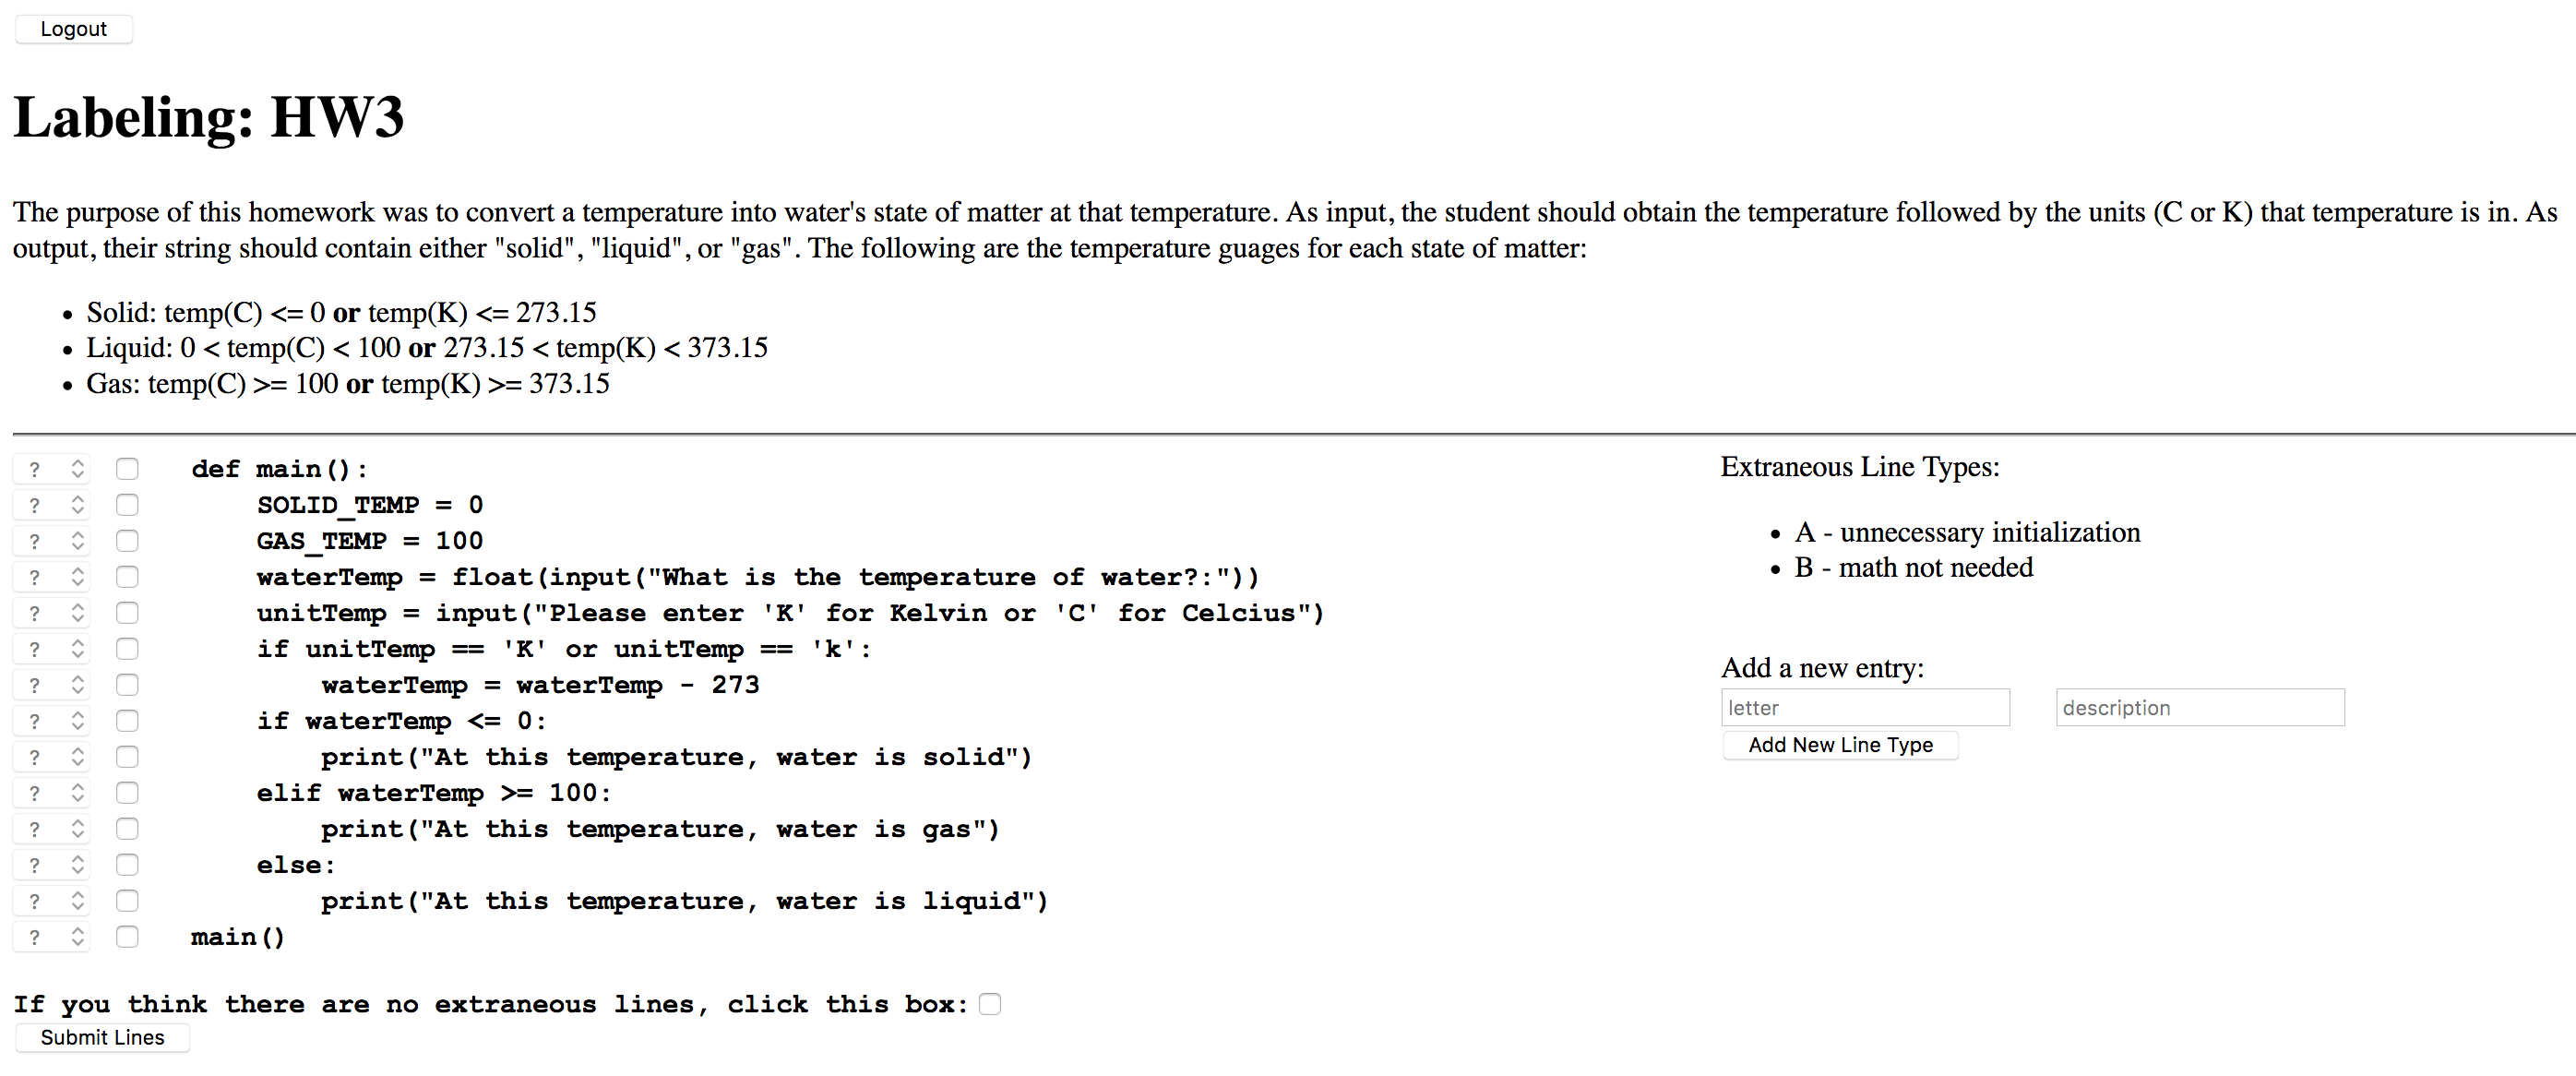
\includegraphics[width=\textwidth]{webapp}
  \caption{Sample screen of a student labeling an assignment.}
  \label{fig:webapp}
\end{figure}

I built a custom web application to standardize the collection of labels. It allows me to easily collect different sets of labels from different people. Each user of the application reads each program, and determines which lines, if any, are extraneous. The application expedites the process of labeling, since navigating between assignments and keeping track of what has already been labeled is taken care of for the user. Figure \ref{fig:webapp} shows a sample screen for a single assignment. On the top of the page, there is a description of the problem, including any guidelines as to what constitutes a correct solution, for their reference. On the left-hand side of the screen, they can view the source code line-by-line. A line is marked as extraneous by clicking a checkbox next to the line in this area and choosing a letter from a drop-down menu. The experts were required to supply a short description of why they marked a line as extraneous. Each expert developed a unique mapping of letter to description to save time in the labeling process. On the right-hand side of the screen they can create a new mappings and view any mappings they have already made. The short description helps me to determine the reliability of each expert labeler. I can compare the lines that multiple experts marked as extraneous, and use the descriptions that the experts provide to verify whether or not that label makes sense. This labeling system contains a few shortcomings that were not discovered or mentioned until after most experts had completed their set of labels. In the interest of full transparency these shortcomings are explained in the following section. 

\subsection{Labeling System Shortcomings}

In this system it was not possible for an expert to label a line with more than one label that they had created. If an expert believed that a line contained multiple transgressions, they had to select the one that they felt was the most relevant instead of marking it with as many labels as possible. This was partly by design, as I did not want an expert to go overboard with  the labeling of any one particular line, but it does prevent the few genuine cases where multiple transgressions were present (by my count, fewer than five such occurrences exist between both problems in my data, i.e., problem 2 number 172 [do I show this code?]) from being accurately labeled. The labeling system also did not allow for existing label letter and description pairs to be edited after they are created. This was less of an issue, as there was no limit on how many pairs that an expert could generate. However, it may have led to some headache during the labeling process if a typo was made or if two lines were similar in fault and the expert did not believe that it needed two different labels. Finally, the design of the web-page itself may have led to some mislabeling. There was some error-checking built into the page itself, such as preventing an expert from submitting a file with no labels without acknowledging that they intend to leave that file unlabeled, and preventing an expert from submitting a line of code as extraneous without a corresponding label. These software checks are unable to catch a mistake in labeling such as accidentally labeling the line directly above or directly underneath your intended line, so the experts had to be careful in their labeling process. 

If I were to redesign the system, I would be sure to include some more data gathering such as the amount of time that a particular expert spends on a single page between arriving on the page and clicking the submit button. This would provide an interesting metric allowing me to gauge how much ``thought'' an expert put into the labeling processing: did they spend a good amount of time reading the solution and thinking about where the extraneous lines, if any, are? Did they just mindlessly click on lines for a short amount of time before moving on to the next file? This is one of the reasons why the selection of trustworthy and capable experts was so important, as this type of data collection is really beyond the scope of this work, but I still require that the labels I am using to understand how well my system performs must be reliable. The following section discusses the reliability and integrity of the expertly-produced labels. 

% Student A - Beatriz
% Student B - Harsh
% Student C - Keith
% Student D - Zoee

\subsection{Label Reliability}

The results of each experiment are heavily influenced by the reliability of the experts who labeled the data. The experts were carefully chosen such that their overall experience would better inform their selection of extraneous lines. To protect the identity of these experts I will refer to them only as Expert A, B, C, or D. Experts A and D are female, while experts B and D are male. Each expert is an undergraduate computer science major who has completed the gateway requirements, meaning that they have all passed the first three introductory courses in the computer science major at UMBC (CMSC 201 - Introductory Programming in Python, CMSC 202 - Object Oriented Programming, and CMSC 341 - Data Structures). Each expert has also served as a teaching assistant for at least one of these introductory courses. In the teaching assistant position, they helped many inexperienced students with homework assignments, and were also responsible for grading those assignments. Having passed the gateway for the major and held a TA position in an introductory course, these experts have experience with identifying lines of code that are not necessary to satisfy the goal of a programming assignment and subsequently giving feedback on those lines.

% Please add the following required packages to your document preamble:
% \usepackage[table,xcdraw]{xcolor}
% If you use beamer only pass "xcolor=table" option, i.e. \documentclass[xcolor=table]{beamer}
% \usepackage[normalem]{ulem}
% \useunder{\uline}{\ul}{}
\begin{table}[h]
\centering
\label{tab:expertLPF}
\begin{tabular}{rrrr}
\multicolumn{1}{l}{} & \multicolumn{1}{l}{{\underline{ \textbf{Lines}}}} & \multicolumn{1}{l}{{\underline{ \textbf{Files}}}} & \multicolumn{1}{l}{{\underline{\textbf{LPF}}}} \\
\rowcolor[HTML]{FFFFC7} 
\multicolumn{1}{l}{\cellcolor[HTML]{FFFFC7}\textbf{Raw Values}} & & & \\
P1 & 8435 & 465 & 18.14 \\
\rowcolor[HTML]{FFFFFF} 
P2 & 6305 & 466 & 13.53 \\
\rowcolor[HTML]{FFFFC7} 
\multicolumn{1}{l}{\cellcolor[HTML]{FFFFC7}\textbf{Expert A}} & 478 & 295 & 1.62 \\
\rowcolor[HTML]{FFFFFF} 
P1 & 138 & 96 & 1.43 \\
\rowcolor[HTML]{EFEFEF} 
P2 & 347 & 199 & 1.73 \\
\rowcolor[HTML]{FFFFC7} 
\multicolumn{1}{l}{\cellcolor[HTML]{FFFFC7}\textbf{Expert B}} & 1276 & 466 & 2.73 \\
\rowcolor[HTML]{FFFFFF} 
P1 & 906 & 263 & 3.44 \\
\rowcolor[HTML]{EFEFEF} 
P2 & 370 & 203 & 1.82 \\
\rowcolor[HTML]{FFFFC7} 
\multicolumn{1}{l}{\cellcolor[HTML]{FFFFC7}\textbf{Expert C}} & 774 & 369 & 2.10 \\
\rowcolor[HTML]{FFFFFF} 
P1 & 575 & 261 & 2.20 \\
\rowcolor[HTML]{EFEFEF} 
P2 & 199 & 107 & 1.86 \\
\rowcolor[HTML]{FFFFC7} 
\multicolumn{1}{l}{\cellcolor[HTML]{FFFFC7}\textbf{Expert D}} & 1092 & 423 & 2.58 \\
\rowcolor[HTML]{FFFFFF} 
P1 & 722 & 211 & 3.42 \\
\rowcolor[HTML]{EFEFEF} 
P2 & 370 & 212 & 1.75 \\
\rowcolor[HTML]{FFFFC7} 
\multicolumn{1}{l}{\cellcolor[HTML]{FFFFC7}\textbf{My Labels}} & 893 & 423 & 2.11 \\
\rowcolor[HTML]{FFFFFF} 
P1 & 481 & 238 & 2.02 \\
\rowcolor[HTML]{EFEFEF} 
P2 & 412 & 223 & 1.85
\end{tabular}
\caption{This shows the amount of lines and files labeled by each of the five experts. LPF stands for Lines Per File. At the top, there is the overall amount of lines and files in the entire data set for comparison.}
\end{table}

Each set of labels produced by an expert will be discussed in the following paragraphs. Table \ref{expertLPF} shows the breakdown of the amount of lines labeled per problem, and the average number of lines labeled per problem, for each set of expert labels. These numbers offer key insights into how each person handled the labeling process. I can compare these numbers to each of the other expert labels, and my own labels, to determine how well each expert created their labels. In this discussion I praise some labels while also offering criticism of other labels. This serves to offer insight into the difficultly and the subjectivity of the labeling process. Each table of expert labels in the following analysis highlights the labels that I believe are the closest in description to labels that I believe should be detectable by my system. All labels produced by the experts are used in the analysis of the experimental results; the criticism of a label does not equate to a removal of that label from the set in order to bolster or diminish the experimental results. 

\vspace{2em}
\bottomcaption{Set of labels produced by Expert A.}\small
\begin{supertabular}{crrl}
\label{labelsA}
Letter & P1 & P2 & Description \\ 
\toprule
A & 73 & 114 & unnecessary conversion of input to string \\
\rowcolor[HTML]{C0C0C0}\textbf{B} &\textbf{ 1} &\textbf{ 3} & \textbf{statement has no effect} \\
\rowcolor[HTML]{C0C0C0} \textbf{C} &\textbf{ 19} &\textbf{ 0} & \textbf{conditional that has no effect} \\
D & 1 & 0 & unnecessary print inside of input \\
\rowcolor[HTML]{C0C0C0} \textbf{E} & \textbf{18} & \textbf{0} & \textbf{statement never reached} \\
F & 10 & 10 & unnecessary conversion of a variable type \\
\rowcolor[HTML]{C0C0C0} \textbf{G} &\textbf{ 1} & \textbf{0} & \textbf{unnecessary variable} \\
H & 2 & 0 & while loop should've been if statement \\
I & 13 & 0 & duplicate code \\
Y & 0 & 202 & unnecessary start and/or step for range function \\
Z & 0 & 18 & loop that only executes once \\
\end{supertabular}
\vspace{2em}

Expert A produced the set of eleven different labels described in Table \ref{labelsA}. Of these labels, I believe that four match up well with my definition of extraneous line of code. This expert describes the liens she found very concisely. She does describe several different cases of statements that don't have any effect, which is exactly the kind of line that I intended for the experts to find. However, this expert labeled the fewest lines per file (LPF) overall. This expert labeled very few files in problem one when compared to each of the other experts, leading to this overall decline in LPF. Accounting for both problems, the type of line that was most identified by this expert concerned an unnecessary start/stop with Python's range() function. This is a common mistake made by novice Python programmers, because there are multiple default behaviors of this function. Some of the lines identified by expert A might not actually be extraneous, such as those with label H or Z. The descriptions of these labels identify a programming construct that was used incorrectly, but that does not mean that the usage of that construct at that particular point was entirely unnecessary to solve the problem. 

Expert B produced the set of twenty different labels described in Table \ref{labelsB}. Half of the labels produced by this expert I believe are well-aligned with my definition of extraneous and should be easily identified by the system. This expert clearly put a substantial amount of effort into the labeling process. They identified the most types of extraneous lines in the data, and they had the highest LPF overall. They were more relaxed in what they understood to be extraneous, as their most identified extraneous line type is simply ``extraneous syntax.'' This label included lines that had unnecessary parentheses, semicolons, and a few other pieces of syntactic sugar that Python understands. At the same time, they were very specific with a selection of their labels. The labels generated by this expert were usually more informative than the other three students, sometimes including information related to a specific problem description. Such labels, however, are not general and will throw off this expert from aligning well with others. The most interesting thing about this expert's labeling is the choice of granularity. They lumped together all extraneous syntax into one category, but split up the same general range() function mistakes into several different categories. 

%\clearpage %force this table to start on the next page
\vspace{5pt}
\bottomcaption{Set of labels produced by Expert B.}
\begin{supertabular}{crrp{.6\textwidth}}
\label{labelsB}
Letter & P1 & P2 & Description \\ 
\toprule
A & 24 & 0 & Constant not used \\
B & 19 & 0 & Extraneous conditional where one or more conditionals have no affect in execution  \\
C & 117 & 122 & Extraneous type cast \\
D & 23 & 0 & Extraneous line duplication \\
E & 86 & 26 & Unnecessary line because it is extra information that does not achieve the program's core functionality requirement \\
F & 3 & 0 & Self Assignment \\
G & 453 & 44 & Extraneous syntax \\
H & 1 & 0 & Unnecessary return \\
I & 159 & 1 & No conditional required or should be default case (i.e. elif is not required if it is the base case)  \\
J & 1 & 0 & This line assumes that water is frozen if the temperature is less than K\_BOIL, which is not true. Water is frozen if below 273 \\
L & 3 & 20 & This operation should not be required \\
M & 6 & 18 & Unnecessary declaration  \\
N & 5 & 0 & Unnecessary operation exit() because using elif will ignore following cases if a previous if statement is true \\
O & 6 & 0 & This value is always overwritten in the following control flow, and is therefore always defined when it is actually used \\
P & 0 & 1 & Range defaults from 0 to n and the 0 is not required \\
Q & 0 & 13 & Unnecessary for loop \\
R & 0 & 2 & Counter not used \\
S & 0 & 11 & The default step of range is 1 \\
T & 0 & 108 & The default start of range is 0 \\
U & 0 & 4 & This function call / declaration does not accomplish anything \\

\end{supertabular}
\vspace{2em}
\clearpage
%\vspace{2em}
\bottomcaption{Set of labels created by Expert C}\small
\begin{supertabular}{crrp{.5\textwidth}}
\label{labelsC}
Letter & P1 & P2 & Description \\ 
\toprule
A & 71 & 37 & unnecessary print \\
B & 18 & 44 & unnecessary initialization \\
C & 66 & 0 & error-handling that does not contribute to solution \\
D & 18 & 6 & unnecessary conditional \\
E & 324 & 1 & an if/elif should be an elif/else \\
F & 71 & 111 & str() used on input() \\
G & 1 & 0 & unnecessary input \\
I & 6 & 0 & exit() not necessary \\

\end{supertabular}
\vspace{2em}

Expert C produced the set of eight different labels described in Table \ref{labelsC}. Of these labels, I believe that six match up very well with my definition of extraneous line of code. This expert understood my definition of extraneous line of code without question, as this ratio is the highest among all of the experts and the difference between their LPF and mine is only .01. However, there is still a point of criticism to be made. The type of line that they identified the most in the data has to due with a mistakenly used programming construct. It seems like the extraneous line marked here is a case of incorrectly applied logic, where the program author is performing an unnecessary test of a condition that could be accomplished with less code. This is a very specific extraneous line that my system may not be able to identify, as the construct is likely still necessary at that point in the solution even though there is a better way to write it that does not require that extra test. The next most identified line by this expert describe an unnecessary type cast on an input statement, similar to each of the other students. Based on their generated labels, I believe that this student had the most accurate internal definition of what it means for a line of code to be extraneous. 

\vspace{2em}
\bottomcaption{Set of labels created by Expert D}\small
\begin{supertabular}{crrp{.5\textwidth}}
\label{labelsD}
Letter & P1 & P2 & Description \\ 
\toprule
A & 2 & 0 & opportunity for compound assignment \\
B & 116 & 124 & unnecessary casting \\
C & 13 & 0 & semicolon to end line \\
D & 2 & 0 & unnecessary return \\
E & 2 & 0 & self assignment \\
F & 560 & 208 & unnecessary parenthesis \\
G & 17 & 6 & added to assignment \\
H & 4 & 0 & Debug statement \\
I & 1 & 0 & condition always true or always false \\
J & 2 & 7 & unused variable \\
K & 2 & 5 & renamed variable \\
L & 1 & 0 & print in input \\
M & 0 & 6 & Always loops once \\
N & 0 & 3 & performs no function \\
O & 0 & 7 & unnecessary initialization \\
P & 0 & 4 & unnecessary parameters \\

\end{supertabular}
\vspace{2em}


Expert D produced the set of sixteen labels described in Table \ref{labelsD}. A little over half of these labels I believe match up well with my definition of extraneous line. Their LPF is only slightly higher than mine, so I believe that this student did understand the general idea. The majority (70\%) of the lines labeled by expert D as described as having ``unnecessary parentheses." Again, the majority of lines marked by this student are extraneous due to a syntax choice rather than an extraneous step in the algorithm. Some of the descriptions provided by this expert are not as informative as they could be, such as ``added to assignment" or ``performs no function." Upon further inspection lines with labels such as these are either just print statements that aren't directly related to the goal of the problem, or some only random statement that is unrelated to the goal. My system should, however, be able to pick up lines aptly labeled ``unused variable" or ``renamed variable" as these may be valid extraneous steps in the algorithm for a particular problem. This expert made a concerted effort to be granular in their labels, but ended up with a few lines types that probably belonged lumped in the same category. 

\begin{table}
\begin{tabular}{crrp{.6\textwidth}}

Letter & P1 & P2 & Description \\ 
\toprule
A & 24 & 8 & variable declared but not used \\
B & 113 & 127 & unnecessary type cast \\
C & 143 & 0 & not necessary to solve problem as described \\
D & 2 & 1 & self assignment \\
E & 2 & 0 & unreachable line of code \\
G & 99 & 0 & else followed immediately by if \\
H & 76 & 26 & extra print statement \\
I & 4 & 0 & same condition tested twice \\
J & 7 & 1 & unnecessary function call \\
K & 9 & 22 & separate variable initialization \\
L & 1 & 0 & string operation not saved \\
M & 1 & 4 & variable reassigned but not altered \\
N & 0 & 192 & range defaults not used properly \\
O & 0 & 16 & loop executes once \\
P & 0 & 6 & counting variable in for loop \\
Q & 0 & 7 & statement has no effect \\
R & 0 & 2 & unneeded function definition \\
\end{tabular}
\caption{Labels created by Student X}
\end{table}


Finally, I produced a set of labels for each of the two assignments in the data set. This baseline was made after all of the experts had created their labels, but before I performed any analysis of what they submitted. I made a few observations during the labeling process that are useful for understanding the general structure and trends lying within the novice code that I used. 

% REORGANIZE THIS SECTION
In the first problem, I found many first-time programmer mistakes. Several students separated the declaration and the initialization steps of creating a variable in Python, which can normally be accomplished in one line. Some students would create a variable with a perfectly relevant name, as if they wanted to use that data purposefully, but then they did not use that variable anywhere else in the program. One of the more prevalent novice issues was the redundant structure of conditional statements; a large amount of students were writing an if statement immediately after an else clause, which is a sequence of statements that could easily be combined if the student consolidated the logic. There were minimal cases, although enough to warrant a mention, of students operating on string variables but not in a way that saved the result of their operation. Strings in python are immutable, therefore if you want to perform an operation you must save the result in a variable with the assignment operator. This is important when a student attempts to force a string to uppercase, or apply any general operation that changes some or all parts of a string. There were students who did not correctly use the input function in their code, instead of passing the prompt string into that function they prompted the user in a separate print statement. A good portion of the students who submitted to this problem included some method of error-checking, or some other code that was semi-related to the problem but not required for their solution to be correct. By the definition of extraneous code that I put forth, these lines should be marked as extraneous as they are not directly related to outputting the correct solution for the problem. One of the most abundant types of extraneous lines involved the casting of data from one type to another. More often than not, the student was casting the result of an input statement to a string; this is redundant as the return value of the input function is already a string. A handful of students were performing mathematical operations inside of the float casting function, this is also redundant as Python will handle the type conversion for you when you write an arithmetic expressions. 

I found the second problem to be remarkably more difficult to label accurately. While there were still many first-time programmer mistakes, there were several more nuanced issues that ended up being marked as extraneous. One such issue is that some students wrote a loop that only executed one time, sometimes the same student would repeatedly write a loop that executed exactly once. This is clearly extraneous as writing that whole construct was unnecessary, the student could remove it and the code would work the same. Many students were just not using the power of iteration to their advantage, and ended up with an extra variable initialization than they really needed (label K). Another nuanced issue was a misuse of the range function, which generates a sequence of integers based on a user-defined start, stop and incremental step. There are default values for the start and the step components of this function, but several students did not take advantage of those values. Instead, they manually entered one or more of those same default values as arguments to the function. This is definitely extraneous, since the default would have been if those arguments were omitted. This problem had a few students who wrote lines of code that I believe were deserving of being marked as multiple types of extraneous lines. However, this is a limitation of the web based labeling application, and I chose the extraneous line type that I thought was the most relevant.

% TODO: ORGANIZE THESE THOUGHTS IN RELIABILITY
\subsubsection{Inter-rater reliability}
Based on the labels produced, each expert clearly had a different internal definition for code that doesn't make sense in the context of a problem. Some experts took a severe approach by including any line of code with inconsequential syntax as extraneous. For example, both sets of labels created by expert B and expert D are dominated by lines of code with unnecessary syntax. Each of the four experts identified some form of unnecessary casting of variable type. There are also instances of experts having a relaxed understanding of extraneous lines of code. For example, <EXAMPLE HERE>. One of the most important things to understand about this labeling process is the distinction between lines of code that do not help the student's solution as it is written, and the lines of code that are just plain incorrect in the same context. Take Problem \#1 solution number 334: [SHOULD I PUT the ACTUAL CODE HERE?].  Table \ref{expert1} shows the breakdown of how those lines in problem 1 were labeled by the experts.  Table \ref{expert2} shows the breakdown of how those lines were labeled by the experts in problem 2.

A noticeable trend in the expert labels is the identification of unnecessary syntax as an extraneous line of code. From the standpoint of the expert, it is clear that lines with extra symbols that do not contribute to the overall solution to the problem should fall within the definition of extraneous line of code. Static code checking tools [CITE PYLINT] already exist to solve this exact problem of unnecessary syntax, and my system is not designed to report such lines. Instead, I am focused on logic and data flow in the novice source code. Therefore, <SHOULD I REMOVE SYNTAX RELATED LABELS?>

Apart from the identification of unnecessary syntax, the experts found a similar set of lines that align with the definition of extraneous code they were provided. Each expert marked lines that contained an unnecessary usage of variable assignment/initialization variables or constructs like ``return" and ``print." A majority of the labels generated by the experts are related to an extraneous use of information like self assignment, or a misuse of logic in the novice source like poor error error handling. Some experts even identified lines of code that do not contribute to the 
    
Some lines end up being marked extraneous by an expert or myself as a means of describing a larger, more fundamental, logical confusion in the solution rather than a single extraneous line. Take label K in Problem 2 for example, it was used to describe a confusion in how for loops use variables, not so much that a declaration was separated from the initialization of a value in the variable itself. 

It is interesting to note that while not every expert labeled more lines overall in the first problem, every expert used more of their labels to cover the first problem than the second. They used a larger spread of unique labels in the first problem, and a tighter spread in the second. For example, expert A has eleven distinct labels that they created, using nine of them to describe lines in the first problem and four of them to describe lines in the second. This trend is true for every expert except for myself, I ended up using an even amount of labels for each problem. This is an intriguing trend to discuss, because I believe that it sheds light on how each expert created their labels. This trend leads me to believe that each expert started by labeling the first problem, creating a set of labels that aligned with the extraneous lines found in that problem. When they finished that problem and moved on to the next one, which is a fundamentally different problem, they found that a majority of the labels that they had created did not fit this new problem at all. They may have also, like me, found problem two to be more difficult to label and overall not have as much room for students to place extraneous lines. So, they would either have had to generate a new label to describe an extraneous line, or figure out which bucket a line fit into best. Thus, their spread of extraneous line types for the second problem was less than the first problem. 


% something similar to the below for every student?
%Although Student A identified almost twice as many unique files for this problem, the average number of lines per file is roughly the same. The culprit seems to be that Student A considers an unnecessary start and/or step in the range() function to be extraneous, as that account for more than half of the lines they identified as extraneous.

\section{Experiments}

%what do I want to test? what is my prediction(s)?
I must perform several experiments to test how well my system performs against the set of expertly-produced labels. The main goal of these experiments is to understand if my system is capable of accurately detecting extraneous lines of code. After testing against the experts, I should be able to answer a few questions: how well is my system able to identify lines that the experts say are extraneous? How well is my system able to identify lines that the experts say are not extraneous? Which combination of line dependency types is the most effective at getting accurate results, if at all? Does changing the combination of line dependency type used have any significant effect on the outcome of the experiment? I hypothesize that the combination of dependencies that uses all three types will be the most accurate of the permutations that I try. I believe this will be the case because of the finer detail afforded by the usage of more dependency types. This should prevent the over-identification of lines that are not actually extraneous, and help to ensure that lines that are actually extraneous are still flagged as such.

In order to answer some of these questions, I need to be able to interchange the types of line dependencies that are being used between experiments. Therefore, the ability to turn different types of dependencies on or off is built into my detection algorithm. A dependency type being ``turned on" means that the detection algorithm is actively using that type of dependency {\color{red}(REFERENCE PRIOR CHAPTER)} to inform its detection of lines in source code. Each experiment reflects one possible combination of line dependency types that are turned on. Different permutations of line dependencies used by the system should help to visualize the impact that different dependency types have on detecting extraneous lines of code. For each problem in the data I will only analyze seven of the eight possible combinations of line dependencies. The case where all three dependency types are turned off in the detection algorithm will be ignored, as that is equivalent to just not running the detection method at all. The rest of the line dependency combinations will be tested so that I have as much information at my disposal to understand how my system performed. I will be able to see how different line dependencies combinations change the ability of the system to identify extraneous liens correctly.I intend to show how different measurements are affected in the progression that starts from the system using a single line dependency type, then adds one more type, and finally adds the last type. 
In order to test the ability of my system to accurately identify extraneous lines, I must compare what it views as extraneous to what the experts view as extraneous. The experts labeled a significant number of individual lines, so in an effort to not crows the analysis I will focus on three versions of the labels that I have: the set of all unique lines that were labeled, the set of lines that were labeled by a majority, and the set of lines that were labeled only by myself. The set of all unique lines that were labeled is the set of lines that were labeled by any expert any amount of times, so a line in this set could have been labeled by a single expert, or it could have been labeled by four different experts. The set of lines labeled by a majority of experts is smaller than the previous set, as it contains lines that were labeled by three or more experts total. I believe that a line of code that has been labeled by the experts in the same manner is more likely to actually be what the experts claim it is, therefore it is more likely that my system will pick up on that same line. I also believe that because I have more intimate knowledge of the system that I should test my system against only the labels that I generated in order to establish how well the other experts did at labeling the data. 

My extraneous line finding system is contained inside of a single class. The instantiation of this class sets up what is necessary to run an experiment with one single combination of line dependency types on a single file. Experimentation with this system therefore involves creating an object of this class with the relevant information, running the detection algorithm on this object, and reporting what is found in the form of a log file. This is done for each assignment in the data. I keep one log file that keeps track of what happens at each step of the algorithm for each assignment that is tested, and I have another solely for reporting the results of each assignment that is experimented with. This allows for ease of creating system performance reports, and for dissecting any individual run for in depth analysis. 

Experimentation with my system is limited by the correctness of each target program. My system is entirely dependent on the completeness and correctness of the target program is it analyzing. For each problem, there are specific student solutions that contain errors. These programs are left out of the following analysis. If the program that I run through my system contains any sort of errors, due to incorrect syntax or otherwise, then I cannot detect extraneous lines in that program. This is a consequence of the dependence on matching the goal output. If a program breaks for any reason, there will not be any output lines that mach the goals of that particular problem. I have defined three classes of errors that I detect and subsequently skip in my system: GoalNotFound, TraceError, and SyntaxError. The GoalNotFound error is an umbrella error thrown when the target program fails to provide output that matches the entire goal for that particular problem. The goal is divided into multiple lines, and if it is not the case that every line has been matched then this error is thrown. The TraceError is thrown when the target program fails for one reason or another during run-time. The leading cause of this error is misinterpretation of the problem instructions by the student, or a failure to submit a complete assignment. The SyntaxError is rather self explanatory, it is an error made by the student responsible for the target program with the syntax of Python. This error outright prevents the student's work from being executed, and is therefore incomplete.

\subsection{Measurements}

I am interested in the performance of each permutation of the algorithm on each of the data sets, and I need to take measurements that can quantify how well the system is able to both identify lines that have been labeled by as expert and lines that have not been identified as extraneous by an expert. The experts were able to label a line as either extraneous (with an accompanying reason) or not label a line meaning that is was not extraneous. My system will state that each line falls into one of these two categories: either it is extraneous or it is not. This means that my system can be treated as a binary classifier. Therefore, a confusion matrix was computed for each run of the algorithm. This captures the amount of correct and incorrect matches between my system and the ground truth labels produced by the experts. The confusion matrix is comprised of four different cases: true positives, false positives, true negatives, and false negatives. Using these four pieces of information, I can calculate how accurate a combination of line dependencies was, how specific and how sensitive the results were, and the F1 score -- an encapsulation of how many false positives and false negatives were in the results. I will now define the preceding terminology in the context of this line labeling problem.

I want the system to correctly identify lines that are considered extraneous by the experts, and to correctly identify lines that are not considered extraneous by the system. Lines labeled by an expert as extraneous are referred to as positive instances, and lines that were not labeled by any expert as extraneous are referred to as negative instances. A true positive (TP) is the case where the system correctly identifies a positive instance, or correctly labels a particular line as extraneous. A true negative (TN) is the case where the system correctly identifies a negative instance, or correctly labels a line as not extraneous. It is important the system is able to identify lines correctly, so both TP and TN results are favorable in the analysis of my system.

The system maybe also incorrectly identify positive and negative instances in the expert labels. A false positive (FP) is the case where a positive instance was incorrectly labeled, or an extraneous line of code (per the experts) was not labeled as extraneous by the system. This means that the system says the line is not necessary in the context of the problem, when in reality it is. A flase negative (FN) is the case where a negative instance was incorrectly labeled, or a line that was not considered extraneous by any expert was considered extraneous by the system. FP and FN results are not favorable and a model classifier should minimize the rate of both such results. The misclassification of extraneous lines would cause much confusion if this system were adopted for use with actual students.

Suppose that the end goal of this classifier were to be placed in a facility where a programming student would interact with the classifier in real time by themselves. It would process a student's solution to a problem, and inform that student of the line number(s) in their code that it believes to be extraneous. If a student were alerted to a line that was a FP, that student would likely be none-the-wiser to that issue. By the definition of extraneous line their code will continue to work as normal; the student would just never be aware of the problem. I believe that a FP result in this context is not harmful to the student, it is the equivalent of the student not using the system in the first place as without the system they also would not know about the extraneous lines that they have written. If a student were alerts to a line that was an FN, that student would be very confused by the system. They would likely an unnecessary amount fo time trying to understand why the line of code 

I believe a false negative result is the more dangerous of the unfavorable results, as the whole idea of the system is to properly identify extraneous lines of code where they exist. A FN represents a complete miss of the purpose of this system.



I would rather the system report that more extraneous lines exist than actually do (report more false positives) than have the system report that less extraneous lines exist than actually do (more false negatives). If this system were to be adopted in an actual introductory computer science class as a supplement to instruction, it would be easier for the trained staff to identify a false positive than a false negative. It is inherently easier for an instructor to tell if a line is not extraneous given that the system believes it to be extraneous. It is not so easy to tell the opposite, if a line that was not labeled should actually have been labeled, at least not at first glance. In any one solution, there will almost always be many more lines that are not extraneous than lines that are extraneous. This is evident in the set of expertly produced labels show in Table \ref{tab:expertLPF}, where each expert labeled anywhere between 1-3 lines per file on average but the solutions for each problem required 18 and 13 lines per file on average respectively. This is by the nature of solving a problem with a program. The implementation of an algorithm requires several lines of code purely in the setup of different constructs, such as loops or conditionals, which increase as the complexity of a problem increases. Therefore, I want to make sure that if a line is marked as not extraneous that the system is almost certain that is the correct choice. The measures of sensitivity and specificity will enable me to be sure that the rate of false positives and false negatives is not too high. 

Specificity in a binary classifier is the ratio of true negative results to the total amount of negative results in the ground truth labels. In the context of my system, specificity is the measure of the ratio of lines that were correctly marked as not extraneous to any line that was marked as not extraneous by the experts. In other words, specificity determines how well your system was able to avoid false alarms in the data. A high specificity would mean that there was a low rate of false positive results, or results that were marked as not extraneous when they should have been marked extraneous. A low specificity means the opposite as the rate of false positives would be higher. Although I argue that the false positive is less important to avoid, this metric should still prove useful when comparing the different permutations of the line dependency types.

Sensitivity in a binary classifier, otherwise known as \emph{recall}, is the ratio of true positive results to the total amount of positive results in the ground truth labels. In the context of my system, sensitivity is the ratio of lines that were correctly labeled by the system to all lines that are considered extraneous by the experts. In other words, recall is a measurement of how well this classifier can detect the positive instances (expert-labeled extraneous lines) in the data. This is a useful calculation to make, as it will allow me to state with some degree of certainty exactly how true a system-labeled extraneous line is. High sensitivity would mean that when my system marked a line as extraneous, it was very sure that line was indeed extraneous. This is equivalent to a low rate of false negatives. A low sensitivity would mean that a line marked extraneous is not particularly trustworthy as there was a large amount of false negative results, or results that were not marked as extraneous but should have been. This is equivalent to a high rate of false negatives. Permutations of the algorithm used by the system that yield high sensitivity are favorable, as that particular permutation would be very certain of the extraneous lines that it marks as such. We want to be sure that we are only labeling the liens that are actually extraneous. I argue that the false negative is a worse error to see in my classifier than a false positive, so achieving a higher sensitivity will be more important in my analysis than achieving a higher specificity.

In addition to sensitivity and specificity, I will measure the precision of each permutation of the algorithm my system uses. This measures the ratio of true positive results to the sum of all results labeled as true by the classifier regardless of correctness(true positives + false positives). In the context of my system, this is a the ratio of system-labeled extraneous lines that are correct to the total amount of system-labeled extraneous lines. This measurement is an answer to a simple question: of all the lines labeled as extraneous by the system, how many were actually extraneous? This is an important measurement to take, because it is a way of making sure that the system is very confident in the lines it is saying are extraneous.

Not only does the nature of the data warrant the calculation of sensitivity and specificity, it also requires that some distinction be made when computing the overall accuracy of the system labels. Normally, the accuracy of a binary classifier is computed as the ratio of correct labels to the total amount of predictions made. However, I am confident that the data will be imbalanced with a larger amount of lines that are not extraneous based solely on the LPF from Table \ref{tab:expertLPF}. Typical accuracy measurement is useless with imbalanced data, particularly when you think that you will perform very well on the task of identifying the side of the imbalance with more data. Therefore, I need a different method of quantifying overall how well my system performed. Overall I would prefer to strike a balance of high sensitivity and specificity to cut down on false positives and false negatives, so I will use a balanced accuracy measure and the F1 Score to do so. The balanced accuracy is the arithmetic mean of sensitivity and specificity, and the F1 score is the harmonic mean of precision and recall. 

\subsection{Problem 1}

% paragraph to describe the setup for the first problem, what was your original prediction? how data will be presented? where were the errors?

\begin{table}[htbp]
\centering

\begin{tabular}{llll}
\multicolumn{1}{l|}{}           & Total        & Error      & Without Error \\ \hline
\multicolumn{1}{l|}{\# Files}   & 465          & 120        & 345           \\
\multicolumn{1}{l|}{\# Lines}   & 8435         & 2221       & 6214          \\
                                &              &            &               \\
\multicolumn{1}{l|}{}           & GoalNotFound & TraceError & SyntaxError   \\ \hline
\multicolumn{1}{l|}{Error Type} & 90           & 22         & 8            
\end{tabular}
\caption{The total amount of files that ran with and without errors for Problem 1, including a breakdown of what errors were seen in the files that were unable to be run through my system. \label{tab:p1FLB}}
\end{table}

The first problem, as described in Table \ref{p1desc}, had 465 total submissions when it was collected to be scored. I was able to include 75\% of those submissions in my experimentation (see Table \ref{tab:p1FLB}) due to errors within these programs. The majority of those not included simply did not submit a correct solution to this problem, which is why there is a large amount of programs showing a GoalNotFound error. A significantly smaller population submitted code that did not work, which is the case for those students falling in the TraceError or SyntaxError categories. 
\begin{table}[htbp]
\centering
\caption{Problem 1 Breakdown}
\begin{tabular}{ll}
\textbf{Agreement By Line} & {Amount} \\
Single Expert       & 632                    \\
Two Experts         & 635                    \\
Three Experts       & 148                     \\
Four Experts        & 44                     \\
Five Experts        & 60                     \\
Total labeled       & 1519                  
\end{tabular}
\caption*{There were 1519 unique lines labels by the experts. This table shows the amount of agreement that exists between them. \label{tab:expert1}}
\end{table}
[TALK ABOUT THE AGREEMENT OF THE EXPERTS FOR PROBLEM ONE HERE. ITS OK.... NOT TOO MANY SINGLE-LABELS BUT STILL NOTICEABLE]

% Please add the following required packages to your document preamble:
% \usepackage[table,xcdraw]{xcolor}
% If you use beamer only pass "xcolor=table" option, i.e. \documentclass[xcolor=table]{beamer}
\begin{table}[htbp]
\centering
\scalebox{0.7}{
\begin{tabular}{rrrrrrrrr}
 &  & \multicolumn{7}{l}{Line Dependency Combination} \\
Consensus & Labels & E & D & S & D+E & E+S & D+S & All \\
\rowcolor[HTML]{EFEFEF} 
One & 423 & 60 (14.18\%) & 401 (95.02\%) & 115 (27.19\%) & 60 (14.18\%) & 54 (12.77\%) & 66 (15.60\%) & 54 (12.77\%) \\
Two & 505 & 128 (25.35\%) & 497 (98.42\%) & 196 (38.81\%) & 128 (25.35\%) & 124 (24.55\%) & 142 (28.12\%) & 124 (24.55\%) \\
\rowcolor[HTML]{EFEFEF} 
Three & 94 & 19 (20.21\%) & 93 (98.94\%) & 61 (64.89\%) & 19 (20.21\%) & 19 (20.21\%) & 35 (37.23\%) & 19 (20.21\%) \\
Four & 28 & 4 (14.29\%) & 27 (96.43\%) & 27 (96.43\%) & 4 (14.29\%) & 3 (10.71\%) & 9 (32.14\%) & 3 (10.71\%) \\
\rowcolor[HTML]{EFEFEF} 
Five & 46 & 2 (4.35\%) & 43 (95.56\%) & 45 (97.83\%) & 2 (4.35\%) & 2 (4.35\%) & 4 (8.70\%) & 2 (4.35\%) \\
Majority & 168 & 25 (14.88\%) & 163 (97.02\%) & 133 (79.17\%) & 25 (14.88\%) & 24 (14.29\%) & 48 (28.57\%) & 24 (12.29\%) \\
\rowcolor[HTML]{EFEFEF} 
Total & 1096 & 213 (19.43\%) & 1061 (96.81\%) & 444 (40.51\%) & 213 (19.43\%) & 202 (18.43\%) & 256 (23.36\%) & 202 (18.43\%)
\end{tabular}}
\end{table} 

% Please add the following required packages to your document preamble:
% \usepackage[table,xcdraw]{xcolor}
% If you use beamer only pass "xcolor=table" option, i.e. \documentclass[xcolor=table]{beamer}
\begin{table}[htbp]
\caption{Problem1 - results with all labels}
\begin{tabular}{c|rrrrlll}
\multicolumn{1}{l|}{Results} & \multicolumn{1}{l}{D} & \multicolumn{1}{l}{E} & \multicolumn{1}{l}{S} & \multicolumn{1}{l}{D+E} & E+S & D+S & All \\ \hline
\rowcolor[HTML]{EFEFEF} 
TP & 1061 & 213 & 444 & 213 & 202 & 256 & 202 \\
FP & 2522 & 358 & 1141 & 358 & 14 & 25 & 14 \\
\rowcolor[HTML]{EFEFEF} 
TN & 2531 & 4760 & 3959 & 4760 & 5104 & 5093 & 5104 \\
FN & 33 & 883 & 648 & 883 & 894 & 840 & 894 \\ \hline
\rowcolor[HTML]{EFEFEF} 
Precision & 0.296 & 0.373 & 0.280 & 0.373 & 0.935 & 0.911 & 0.935 \\
Sensitivity & 0.970 & 0.194 & 0.407 & 0.194 & 0.184 & 0.234 & 0.184 \\
\rowcolor[HTML]{EFEFEF} 
Specificity & 0.501 & 0.930 & 0.776 & 0.930 & 0.997 & 0.995 & 0.997 \\
\multicolumn{1}{l|}{Accuracy} & \multicolumn{1}{l}{0.584} & \multicolumn{1}{l}{0.800} & \multicolumn{1}{l}{0.711} & \multicolumn{1}{l}{0.800} & 0.854 & 0.861 & 0.854 \\
\rowcolor[HTML]{EFEFEF} 
\multicolumn{1}{l|}{\cellcolor[HTML]{EFEFEF}\begin{tabular}[c]{@{}l@{}}Balanced\\ Accuracy\end{tabular}} & \multicolumn{1}{l}{\cellcolor[HTML]{EFEFEF}0.735} & \multicolumn{1}{l}{\cellcolor[HTML]{EFEFEF}0.562} & \multicolumn{1}{l}{\cellcolor[HTML]{EFEFEF}0.591} & \multicolumn{1}{l}{\cellcolor[HTML]{EFEFEF}0.562} & 0.591 & 0.614 & 0.591 \\
\multicolumn{1}{l|}{F1 Score} & \multicolumn{1}{l}{0.454} & \multicolumn{1}{l}{0.256} & \multicolumn{1}{l}{0.332} & \multicolumn{1}{l}{0.256} & 0.308 & 0.372 & 0.308
\end{tabular}
\end{table}

% Please add the following required packages to your document preamble:
% \usepackage[table,xcdraw]{xcolor}
% If you use beamer only pass "xcolor=table" option, i.e. \documentclass[xcolor=table]{beamer}
\begin{table}[htbp]
\caption{problem 1 - results with majority labels}
\begin{tabular}{c|rrrrlll}
\multicolumn{1}{l|}{Results} & \multicolumn{1}{l}{D} & \multicolumn{1}{l}{E} & \multicolumn{1}{l}{S} & \multicolumn{1}{l}{D+E} & E+S & D+S & All \\ \hline
\rowcolor[HTML]{EFEFEF} 
TP & 163 & 25 & 133 & 25 & 24 & 48 & 24 \\
FP & 3420 & 546 & 1452 & \textbf{546} & 192 & 233 & 192 \\
\rowcolor[HTML]{EFEFEF} 
TN & 2560 & 5500 & 4573 & 5500 & 5854 & 5813 & 5854 \\
FN & 4 & 143 & 34 & 143 & 144 & 120 & 144 \\ \hline
\rowcolor[HTML]{EFEFEF} 
Precision & 0.045 & 0.044 & 0.084 & 0.044 & 0.111 & 0.171 & 0.111 \\
Sensitivity & 0.976 & 0.149 & 0.796 & 0.149 & 0.143 & 0.286 & 0.143 \\
\rowcolor[HTML]{EFEFEF} 
Specificity & 0.428 & 0.910 & 0.759 & 0.910 & 0.968 & 0.961 & 0.968 \\
Accuracy & \multicolumn{1}{l}{0.443} & \multicolumn{1}{l}{0.889} & \multicolumn{1}{l}{0.760} & \multicolumn{1}{l}{0.889} & 0.946 & 0.943 & 0.946 \\
\rowcolor[HTML]{EFEFEF} 
\begin{tabular}[c]{@{}r@{}}Balanced\\ Accuracy\end{tabular} & \multicolumn{1}{l}{\cellcolor[HTML]{EFEFEF}0.702} & \multicolumn{1}{l}{\cellcolor[HTML]{EFEFEF}0.529} & \multicolumn{1}{l}{\cellcolor[HTML]{EFEFEF}0.778} & \multicolumn{1}{l}{\cellcolor[HTML]{EFEFEF}0.529} & 0.556 & 0.624 & 0.556 \\
F1 Score & \multicolumn{1}{l}{0.087} & \multicolumn{1}{l}{0.068} & \multicolumn{1}{l}{0.152} & \multicolumn{1}{l}{0.068} & 0.125 & 0.214 & 0.125
\end{tabular}
\end{table}

% Please add the following required packages to your document preamble:
% \usepackage[table,xcdraw]{xcolor}
% If you use beamer only pass "xcolor=table" option, i.e. \documentclass[xcolor=table]{beamer}
\begin{table}[htbp]
\caption{problem 1 - results with just michael`s labels}
\begin{tabular}{r|rrrrlll}
\multicolumn{1}{l|}{Results} & \multicolumn{1}{l}{D} & \multicolumn{1}{l}{E} & \multicolumn{1}{l}{S} & \multicolumn{1}{l}{D+E} & E+S & D+S & All \\ \hline
\rowcolor[HTML]{EFEFEF} 
TP & 336 & 190 & 328 & 190 & 188 & 237 & 188 \\
FP & 3247 & 381 & 1257 & \textbf{381} & 28 & 44 & 28 \\
\rowcolor[HTML]{EFEFEF} 
TN & 2560 & 5492 & 4595 & 5492 & 5845 & 5829 & 5845 \\
FN & 4 & 151 & 12 & 151 & 153 & 104 & 153 \\ \hline
\rowcolor[HTML]{EFEFEF} 
Precision & 0.094 & 0.333 & \textbf{0.207} & 0.333 & 0.870 & 0.843 & 0.870 \\
Sensitivity & 0.988 & 0.557 & 0.965 & \textbf{0.557} & 0.551 & 0.695 & 0.551 \\
\rowcolor[HTML]{EFEFEF} 
Specificity & 0.441 & 0.935 & \textbf{0.785} & 0.935 & 0.995 & 0.993 & 0.995 \\
\multicolumn{1}{l|}{Accuracy} & \multicolumn{1}{l}{0.471} & \multicolumn{1}{l}{0.914} & \multicolumn{1}{l}{.795} & \multicolumn{1}{l}{0.914} & 0.971 & 0.976 & 0.971 \\
\rowcolor[HTML]{EFEFEF} 
\multicolumn{1}{l|}{\cellcolor[HTML]{EFEFEF}\begin{tabular}[c]{@{}l@{}}Balanced\\ Accuracy\end{tabular}} & \multicolumn{1}{l}{\cellcolor[HTML]{EFEFEF}0.715} & \multicolumn{1}{l}{\cellcolor[HTML]{EFEFEF}0.746} & \multicolumn{1}{l}{\cellcolor[HTML]{EFEFEF}0.875} & \multicolumn{1}{l}{\cellcolor[HTML]{EFEFEF}0.746} & 0.773 & 0.844 & 0.773 \\
\multicolumn{1}{l|}{F1 Score} & \multicolumn{1}{l}{0.171} & \multicolumn{1}{l}{0.675} & \multicolumn{1}{l}{0.341} & \multicolumn{1}{l}{0.417} & 0.675 & 0.762 & 0.675
\end{tabular}
\end{table}

\subsubsection{Analysis}
Stuff goes here.

% was your prediction confirmed or denied with this problem? 

\subsection{Problem 2}

\begin{table}[htbp]
\centering
\begin{tabular}{lllll}
\multicolumn{1}{l|}{}           & Total        & Error      & Without Error &       \\ \cline{1-4}
\multicolumn{1}{l|}{\# Files}   & 466          & 68         & 398           &       \\
\multicolumn{1}{l|}{\# Lines}   & 6305         & 924        & 5381          &       \\
                                &              &            &               &       \\
\multicolumn{1}{l|}{}           & GoalNotFound & TraceError & SyntaxError   & Other \\ \hline
\multicolumn{1}{l|}{Error Type} & 49           & 9          & 9             & 1    
\end{tabular}
\caption{The total amount of files that ran with and without errors for Problem 2, including a breakdown of what errors were seen in the files that were unable to be run through my system.}
\end{table}

This is where I describe the setup for the second problem.

% Please add the following required packages to your document preamble:
% \usepackage[table,xcdraw]{xcolor}
% If you use beamer only pass "xcolor=table" option, i.e. \documentclass[xcolor=table]{beamer}
\begin{table}[htbp]
\centering
\scalebox{0.7}{
\begin{tabular}{lllllllll}
 &  & \multicolumn{7}{c}{Line Dependency Combination} \\ \hline
\multicolumn{1}{|l|}{Consensus} & \multicolumn{1}{l|}{Labels} & \multicolumn{1}{l|}{E} & \multicolumn{1}{l|}{D} & \multicolumn{1}{l|}{S} & \multicolumn{1}{l|}{D+E} & \multicolumn{1}{l|}{E+S} & \multicolumn{1}{l|}{D+S} & \multicolumn{1}{l|}{All} \\ \hline
\rowcolor[HTML]{EFEFEF} 
\multicolumn{1}{|l|}{\cellcolor[HTML]{EFEFEF}One} & \multicolumn{1}{l|}{\cellcolor[HTML]{EFEFEF}260} & \multicolumn{1}{l|}{\cellcolor[HTML]{EFEFEF}10(3.85\%)} & \multicolumn{1}{l|}{\cellcolor[HTML]{EFEFEF}171 (65.77\%)} & \multicolumn{1}{l|}{\cellcolor[HTML]{EFEFEF}129 (49.62\%)} & \multicolumn{1}{l|}{\cellcolor[HTML]{EFEFEF}8 (3.08\%)} & \multicolumn{1}{l|}{\cellcolor[HTML]{EFEFEF}10 (3.85\%)} & \multicolumn{1}{l|}{\cellcolor[HTML]{EFEFEF}34 (13.18\%)} & \multicolumn{1}{l|}{\cellcolor[HTML]{EFEFEF}8 (3.08\%)} \\ \cline{5-5} \cline{7-7} \cline{9-9} 
\multicolumn{1}{|l|}{Two} & \multicolumn{1}{l|}{132} & \multicolumn{1}{l|}{17(12.88\%)} & \multicolumn{1}{l|}{112 (84.85\%)} & \multicolumn{1}{l|}{64 (50.00\%)} & \multicolumn{1}{l|}{9 (6.82\%)} & \multicolumn{1}{l|}{17 (12.88\%)} & \multicolumn{1}{l|}{25 (19.08\%)} & \multicolumn{1}{l|}{9 (6.82\%)} \\ \cline{1-1} \cline{5-5} \cline{7-7} \cline{9-9} 
\rowcolor[HTML]{EFEFEF} 
\multicolumn{1}{|l|}{\cellcolor[HTML]{EFEFEF}Three} & \multicolumn{1}{l|}{\cellcolor[HTML]{EFEFEF}107} & \multicolumn{1}{l|}{\cellcolor[HTML]{EFEFEF}5 (4.67\%)} & \multicolumn{1}{l|}{\cellcolor[HTML]{EFEFEF}104 (97.20\%)} & \multicolumn{1}{l|}{\cellcolor[HTML]{EFEFEF}42 (39.25\%)} & \multicolumn{1}{l|}{\cellcolor[HTML]{EFEFEF}5 (4.67\%)} & \multicolumn{1}{l|}{\cellcolor[HTML]{EFEFEF}5 (4.67\%)} & \multicolumn{1}{l|}{\cellcolor[HTML]{EFEFEF}18 (16.82\%)} & \multicolumn{1}{l|}{\cellcolor[HTML]{EFEFEF}5 (4.67\%)} \\ \cline{5-5} \cline{7-7} \cline{9-9} 
\multicolumn{1}{|l|}{Four} & \multicolumn{1}{l|}{33} & \multicolumn{1}{l|}{14 (42.42\%)} & \multicolumn{1}{l|}{15 (45.45\%)} & \multicolumn{1}{l|}{25 (75.76\%)} & \multicolumn{1}{l|}{1 (3.03\%)} & \multicolumn{1}{l|}{14 (42.42\%)} & \multicolumn{1}{l|}{7 (22.58\%)} & \multicolumn{1}{l|}{1 (3.03\%)} \\ \cline{5-5} \cline{7-7} \cline{9-9} 
\rowcolor[HTML]{EFEFEF} 
\multicolumn{1}{|l|}{\cellcolor[HTML]{EFEFEF}Five} & \multicolumn{1}{l|}{\cellcolor[HTML]{EFEFEF}85} & \multicolumn{1}{l|}{\cellcolor[HTML]{EFEFEF}83 (97.65\%)} & \multicolumn{1}{l|}{\cellcolor[HTML]{EFEFEF}6 (7.06\%)} & \multicolumn{1}{l|}{\cellcolor[HTML]{EFEFEF}83 (97.65\%)} & \multicolumn{1}{l|}{\cellcolor[HTML]{EFEFEF}0} & \multicolumn{1}{l|}{\cellcolor[HTML]{EFEFEF}83 (97.65\%)} & \multicolumn{1}{l|}{\cellcolor[HTML]{EFEFEF}4 (4.71\%)} & \multicolumn{1}{l|}{\cellcolor[HTML]{EFEFEF}0} \\ \cline{5-5} \cline{7-7} \cline{9-9} 
\multicolumn{1}{|l|}{Majority} & \multicolumn{1}{l|}{225} & \multicolumn{1}{l|}{102 (45.33\%)} & \multicolumn{1}{l|}{125 (55.56\%)} & \multicolumn{1}{l|}{150 (66.67\%)} & \multicolumn{1}{l|}{6 (2.67\%)} & \multicolumn{1}{l|}{102 (45.33\%)} & \multicolumn{1}{l|}{29 (13\%)} & \multicolumn{1}{l|}{6 (2.67\%)} \\ \cline{5-5} \cline{7-7} \cline{9-9} 
\rowcolor[HTML]{EFEFEF} 
\multicolumn{1}{|l|}{\cellcolor[HTML]{EFEFEF}Total} & \multicolumn{1}{l|}{\cellcolor[HTML]{EFEFEF}617} & \multicolumn{1}{l|}{\cellcolor[HTML]{EFEFEF}129 (20.91\%)} & \multicolumn{1}{l|}{\cellcolor[HTML]{EFEFEF}408 (66.13\%)} & \multicolumn{1}{l|}{\cellcolor[HTML]{EFEFEF}343 (55.95\%)} & \multicolumn{1}{l|}{\cellcolor[HTML]{EFEFEF}23 (3.73\%)} & \multicolumn{1}{l|}{\cellcolor[HTML]{EFEFEF}129 (20.91\%)} & \multicolumn{1}{l|}{\cellcolor[HTML]{EFEFEF}88 (14.38\%)} & \multicolumn{1}{l|}{\cellcolor[HTML]{EFEFEF}23 (3.73\%)} \\ \cline{3-3} \cline{5-5} \cline{7-7} \cline{9-9} 
\end{tabular}}
\end{table}

% Please add the following required packages to your document preamble:
% \usepackage[table,xcdraw]{xcolor}
% If you use beamer only pass "xcolor=table" option, i.e. \documentclass[xcolor=table]{beamer}
\begin{table}[htbp]
\caption{problem 2 - results with majority labels}
\begin{tabular}{r|rrrrlll}
\multicolumn{1}{l|}{Results majority} & \multicolumn{1}{l}{D} & \multicolumn{1}{l}{E} & \multicolumn{1}{l}{S} & \multicolumn{1}{l}{D+E} & E+S & D+S & All \\ \hline
\rowcolor[HTML]{EFEFEF} 
TP & 125 & 102 & 120 & 6 & 102 & 29 & 6 \\
FP & 1879 & 1042 & 2454 & \textbf{343} & 802 & 335 & 103 \\
\rowcolor[HTML]{EFEFEF} 
TN & 3266 & 4114 & 2680 & 4813 & 4354 & 4791 & 5053 \\
FN & 100 & 123 & 75 & 219 & 123 & 194 & 219 \\ \hline
\rowcolor[HTML]{EFEFEF} 
Precision & 0.062 & 0.089 & \textbf{0.058} & 0.017 & 0.113 & 0.080 & 0.055 \\
Sensitivity & 0.556 & 0.453 & 0.667 & \textbf{0.027} & 0.453 & 0.130 & 0.027 \\
\rowcolor[HTML]{EFEFEF} 
Specificity & 0.635 & 0.798 & \textbf{0.522} & 0.933 & 0.844 & 0.935 & 0.980 \\
\multicolumn{1}{l|}{Accuracy} & \multicolumn{1}{l}{0.631} & \multicolumn{1}{l}{0.783} & \multicolumn{1}{l}{0.528} & \multicolumn{1}{l}{0.896} & 0.828 & 0.901 & 0.940 \\
\rowcolor[HTML]{EFEFEF} 
\multicolumn{1}{l|}{\cellcolor[HTML]{EFEFEF}\begin{tabular}[c]{@{}l@{}}Balanced\\ Accuracy\end{tabular}} & \multicolumn{1}{l}{\cellcolor[HTML]{EFEFEF}0.595} & \multicolumn{1}{l}{\cellcolor[HTML]{EFEFEF}0.626} & \multicolumn{1}{l}{\cellcolor[HTML]{EFEFEF}0.594} & \multicolumn{1}{l}{\cellcolor[HTML]{EFEFEF}0.480} & 0.649 & 0.532 & 0.503 \\
\multicolumn{1}{l|}{F1 Score} & \multicolumn{1}{l}{0.112} & \multicolumn{1}{l}{0.149} & \multicolumn{1}{l}{0.106} & \multicolumn{1}{l}{0.021} & 0.181 & 0.099 & 0.036
\end{tabular}
\end{table}

% Please add the following required packages to your document preamble:
% \usepackage[table,xcdraw]{xcolor}
% If you use beamer only pass "xcolor=table" option, i.e. \documentclass[xcolor=table]{beamer}
\begin{table}[htbp]
\caption{problem 2 - results with all labels}
\begin{tabular}{r|rrrrlll}
\multicolumn{1}{l|}{Results overall} & \multicolumn{1}{l}{D} & \multicolumn{1}{l}{E} & \multicolumn{1}{l}{S} & \multicolumn{1}{l}{D+E} & E+S & D+S & All \\ \hline
\rowcolor[HTML]{EFEFEF} 
TP & 408 & 129 & 343 & 23 & 129 & 88 & 23 \\
FP & 1596 & 1015 & 2261 & \textbf{326} & 775 & 276 & 86 \\
\rowcolor[HTML]{EFEFEF} 
TN & 3159 & 3751 & 2487 & 4440 & 3991 & 4463 & 4680 \\
FN & 207 & 486 & 268 & 592 & 486 & 522 & 592 \\ \hline
\rowcolor[HTML]{EFEFEF} 
Precision & 0.204 & 0.113 & \textbf{0.132} & 0.066 & 0.143 & 0.242 & 0.211 \\
Sensitivity & 0.663 & 0.210 & 0.561 & \textbf{0.037} & 0.210 & 0.144 & 0.037 \\
\rowcolor[HTML]{EFEFEF} 
Specificity & 0.664 & 0.787 & \textbf{0.524} & 0.932 & 0.837 & 0.942 & 0.982 \\
\multicolumn{1}{l|}{Accuracy} & \multicolumn{1}{l}{0.664} & \multicolumn{1}{l}{0.721} & \multicolumn{1}{l}{0.528} & \multicolumn{1}{l}{0.829} & 0.766 & 0.851 & 0.874 \\
\rowcolor[HTML]{EFEFEF} 
\multicolumn{1}{l|}{\cellcolor[HTML]{EFEFEF}\begin{tabular}[c]{@{}l@{}}Balanced\\ Accuracy\end{tabular}} & \multicolumn{1}{l}{\cellcolor[HTML]{EFEFEF}0.664} & \multicolumn{1}{l}{\cellcolor[HTML]{EFEFEF}0.498} & \multicolumn{1}{l}{\cellcolor[HTML]{EFEFEF}0.543} & \multicolumn{1}{l}{\cellcolor[HTML]{EFEFEF}0.484} & 0.524 & 0.543 & 0.510 \\
\multicolumn{1}{l|}{F1 Score} & \multicolumn{1}{l}{0.312} & \multicolumn{1}{l}{0.147} & \multicolumn{1}{l}{0.213} & \multicolumn{1}{l}{0.048} & 0.170 & 0.181 & 0.064
\end{tabular}
\end{table}

% Please add the following required packages to your document preamble:
% \usepackage[table,xcdraw]{xcolor}
% If you use beamer only pass "xcolor=table" option, i.e. \documentclass[xcolor=table]{beamer}
\begin{table}[htbp]
\caption{problem 2 - results with just michael's labels}
\begin{tabular}{r|rrrrlll}
\multicolumn{1}{l|}{Results} & \multicolumn{1}{l}{D} & \multicolumn{1}{l}{E} & \multicolumn{1}{l}{S} & \multicolumn{1}{l}{D+E} & E+S & D+S & All \\ \hline
\rowcolor[HTML]{EFEFEF} 
TP & 220 & 108 & 212 & 12 & 108 & 59 & 12 \\
FP & 1784 & 1036 & 2392 & \textbf{337} & 796 & 305 & 97 \\
\rowcolor[HTML]{EFEFEF} 
TN & 3250 & 4009 & 2635 & 4708 & 4249 & 4713 & 4948 \\
FN & 116 & 228 & 120 & 324 & 228 & 272 & 324 \\ \hline
\rowcolor[HTML]{EFEFEF} 
Precision & 0.110 & 0.094 & \textbf{0.081} & 0.034 & 0.119 & 0.162 & 0.110 \\
Sensitivity & 0.655 & 0.321 & 0.639 & \textbf{0.036} & 0.321 & 0.178 & 0.036 \\
\rowcolor[HTML]{EFEFEF} 
Specificity & 0.646 & 0.795 & \textbf{0.524} & 0.933 & 0.842 & 0.939 & 0.981 \\
\multicolumn{1}{l|}{Accuracy} & \multicolumn{1}{l}{0.646} & \multicolumn{1}{l}{0.765} & \multicolumn{1}{l}{0.531} & \multicolumn{1}{l}{0.877} & 0.810 & 0.892 & 0.922 \\
\rowcolor[HTML]{EFEFEF} 
\multicolumn{1}{l|}{\cellcolor[HTML]{EFEFEF}\begin{tabular}[c]{@{}l@{}}Balanced\\ Accuracy\end{tabular}} & \multicolumn{1}{l}{\cellcolor[HTML]{EFEFEF}0.650} & \multicolumn{1}{l}{\cellcolor[HTML]{EFEFEF}0.558} & \multicolumn{1}{l}{\cellcolor[HTML]{EFEFEF}0.581} & \multicolumn{1}{l}{\cellcolor[HTML]{EFEFEF}0.484} & 0.582 & 0.559 & 0.508 \\
\multicolumn{1}{l|}{F1 Score} & \multicolumn{1}{l}{0.188} & \multicolumn{1}{l}{0.146} & \multicolumn{1}{l}{0.144} & \multicolumn{1}{l}{0.035} & 0.174 & 0.170 & 0.054
\end{tabular}
\end{table}


\subsubsection{Analysis}
%This is where I talk about specific intuitions regarding the second problem.
Stuff goes here. 

\section{Conclusion}

The problem of accurately identifying the presence of an extraneous line of code in a program written by a novice student is incredibly complex. 

\subsection{Future work?}

\end{document}
